\subsection{MPEG-2 Motion Estimation}
\label{sec:mpeg}

\begin{figure}[t]
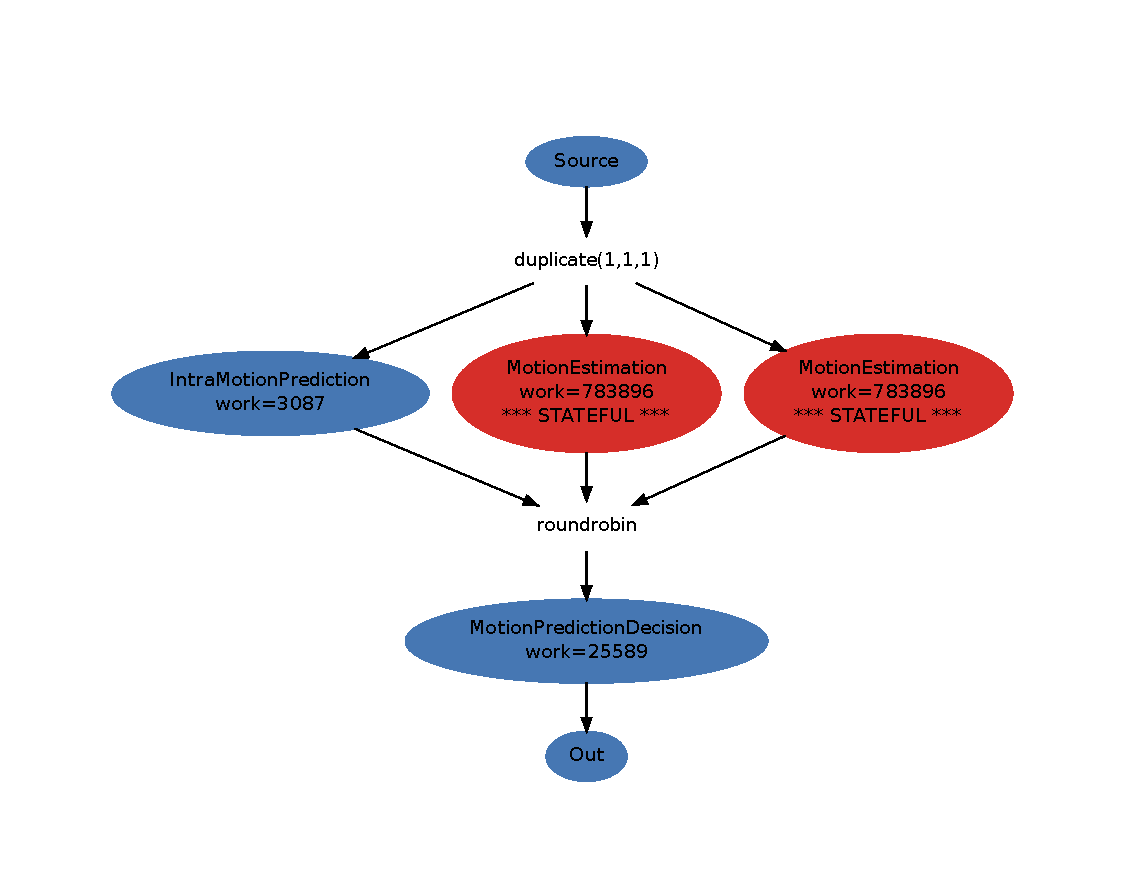
\includegraphics[width=3.3in]{figures/work_estimate_mpeg_motionestimation.pdf}
\caption{MPEG Motion Estimation stream graph.\protect\label{fig:mpegMEgraph}}
\end{figure}


This section presents an application of induction variables to the Motion Estimation compression subset of the MPEG-2 encoder.  MPEG-2 is a standard for coding moving pictures and audio information and has a wide variety of multimedia applications.  

The specification contains various types of compression, one of which is motion prediction.  Motion prediction takes advantage of the fact that frames of a video contain a large amount of duplicated scenes between consecutive frames.  Motion estimation attempts to generate predictions with respect to a set of reference frames obtained from previous or future pictures.  Accordingly, the MPEG-2 encoder can utilize forward and backward motion estimation to achieve this form of compression.  The process of Motion Estimation entails comparing pixel blocks between frames and forming a motion vector indicating a cartesian displacement of a macroblock between reference frames.  

The Motion estimation stream subgraph of the MPEG-2 encoder is illustrated in Figure~\ref{fig:mpegMEgraph}~\cite{drake-thesis}.  Each block of pixels will be tested against three types of prediction (no prediction, forward predicted, and backward predicted) to determine which is the best method for motion estimation.  The MotionEstimationDecision filter determines which is the best encoding technique for this macroblock.

The work estimation of this compression indicates the filter MotionEstimation is stateful and contains the majority of the work.  The MotionEstimation filter pulls macroblocks at a time, iterating through a two-dimensional array (16x16 macroblocks) along the picture.  The filter relies on induction variables to maintain its array position.  We can apply the induction variable transformation on this filter to remove the state in the filter.

Reference pictures are set using upstream messaging from later in the stream graph.  Currently the backend does not support the use of upstream messaging, so for the purpose of benchmarking this application, the reference picture is set to a dummy value and is unchanged throughout the program.  This does not detract from the data parallelism introduced after removing the induction state.  Upstream messaging would simply require that sent messages be duplicated to all fissed filters in the stream graph.

\begin{figure}[t]
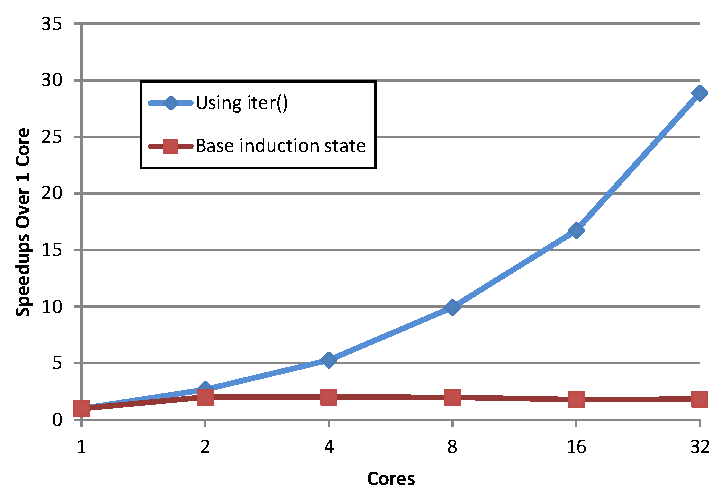
\includegraphics[width=3.3in]{figures/mpeg-results.pdf}
\caption{Speedups for MPEG-2 Encoder Motion Estimation subset, with and without induction variable state.  \protect\label{fig:mpeg-results}}
\end{figure}

Figure~\ref{fig:mpeg-results} shows the runtime figures for the original stateful MPEG-2 motion estimation subset compared to the stateless subset.  We can see significant improvements to runtime after making this subset stateless and exposing data parallelism.